\section{Aufgabe 1-3}
Bei dieser Aufgabe werden vor allem Einstellungen gesucht, bei denen eine Aufnahme der Franck-Hertz-Kurve in möglichst schöner Form möglich sind. Dabei hängt das Aussehen der Kurve von verschiedenen Faktoren ab. Verwendet werden ein Funktionsgeneartor, der folgende Parameter bestimmt:
\begin{itemize}
\item[] \textbf{Heizspannung:} Da die Heizspannung für ein Austreten von Elektronen aus der Kathode sorgt, gibt es einen Zusammenhang zwischen dem Strom von Anode zu Gegenkathode \(I\) und der Heizspannung \(U_H\). Es ist eine genügend große Heizspannung zu wählen, um ein Austreten von Elektronen zu ermöglichen, ist diese erreicht, hat eine weitere Erhöhung nur noch wenig Effekt, sorgt im Allgemeinen aber für eine Erhöhung des Stroms \(I\).
\item[] \textbf{Beschleunigungsspannung:} Die Beschleunigungsspannunng ist die Spannung \(U_B\), die zweischen Anode und Kathode angelegt wird. Sie sorgt dafür, dass sich die Elektronen in einem Elektrischen Feld befinden und somit \textit{beschleunigt} werden.

Bei diesem Versuchsaufbau wird die Beschleunigungsspannung variiert, indem eine Wechselspannung verwendet wird.

\item[] \textbf{Temperatur:} Die Temperatur wird bei dem vorhandenen Versuchsaufbau eingestellt, indem ein Thermostat an der Apparatur selbst eingestellt wird, welches eine elektrische Heizung steuert. Da das Thermostat sehr langsam reagiert, ist es sehr schwer die Temperatur genau einzustellen. Sie ändert sich also während einer Messung erheblich.

Sie sorgt dafür, dass das Quecksilber in den gasförmigen Zustand übergeht, da sonst kein ausreichender Abstand der Atome gegeben ist.
\end{itemize}
\subsection{Aufbau}
Der Aufbau wurde schon fertig vorgefunden. Es werden daher nur alle Steckverbindungen auf deren Richtigkeit überprüft, die Geräte eingeschaltet und der Computer für die Aufnahme der Messwerte hochgefahren. Verwendet werden die Frank-Hertz-Röhre mit Heizthermostat und Heizung, ein USB-Oszilloskop für den Computer und ein speziell für den Franck-Hertz-Versuch gefertigtes Netzteil für die Spannungsversorgung der Apparatur. Anschließend wird mit der Durchführung begonnen.
\subsection{Durchführung}
Im Rahmen der ersten Aufgabe wurde zunächst eine Einstellung gesucht, bei der im X-Y-Bild ein möglichst gut erkennbarer Kurvenverlauf sichtbar wurde. Angezeigt wurde \(I\) über \(U_B\), wobei \(I\) nicht exakt gemessen wird, sondern nur eine proportionale Spannung über einen Widerstand detektiert wurde. Aufgrund eines Hinweises des leitenden Tutors, wurde dahingehend von der Aufgabenstellung abgewichen, dass Kurven für \(155, 185, 205\, ^\circ C\) aufgenommen wurden, da diese leichter zu messen sind.
\subsection{Fehlerbetrachtung}
Die Fehler der Messung ist im Allgemeinen nur schwer anzugeben, daher werden die Fehler der Steigungen aus der Streuung berechnet. Das USB-Oszilloskop hat eine begrenzte Auflösung, was man an der Rasterstruktur der Messwerte sehen kann. Außerdem streuen die Messwerte auch erheblich, was an den breiten Kurven zu sehen ist. Des weiteren sind auch diverse systematische Fehler vorhanden gewesen, z.B. wurde um die Spannung zu messen, ein Spannungsteiler verwendet, der den Messwert weiter verfälscht.
\subsection{Graphen/Messwerte}
Die Messdaten wurden als Textdatei aus dem Programm exportiert und anschließend mit GNU-Plot dargestellt. Dabei wurde der Faktor 10 für die echte Spannung für \(U_B\) berücksichtigt. Die Minima wurden nur mit Augenmaß geschätzt, da ein Kurven-\textit{fitting} aufgrund der  breiten Streuung der Messwerte nicht möglich war. 
\begin{center}
\begin{minipage}{\linewidth}
\centering
\makebox[0cm]{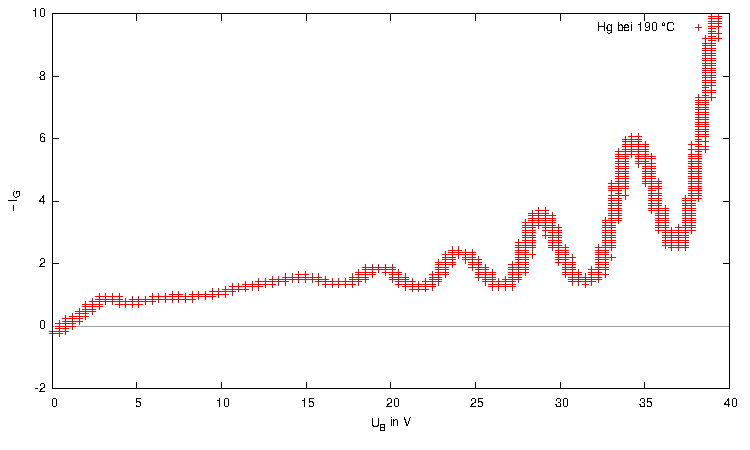
\includegraphics[width=\textwidth]{graphen/a1/a1}}
\captionof{figure}{Erste für A2 aufgenommene Franck-Hertz-Kurve (\(T=190\,^\circ C\))}
\label{a1}
\end{minipage}
\begin{minipage}{\linewidth}
\centering
\makebox[0cm]{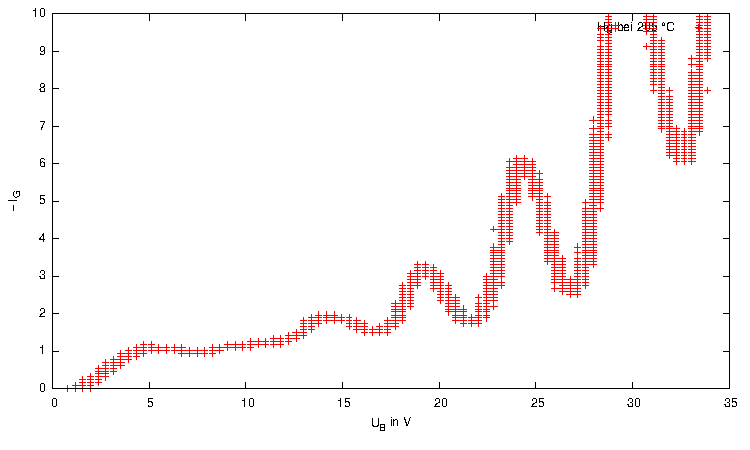
\includegraphics[width=\textwidth]{graphen/a2/a2c}}
\captionof{figure}{Erste für A3 aufgenommene Franck-Hertz-Kurve (\(T=155\,^\circ C\))}
\label{a2a}
\end{minipage}
\begin{minipage}{\linewidth}
\centering
\makebox[0cm]{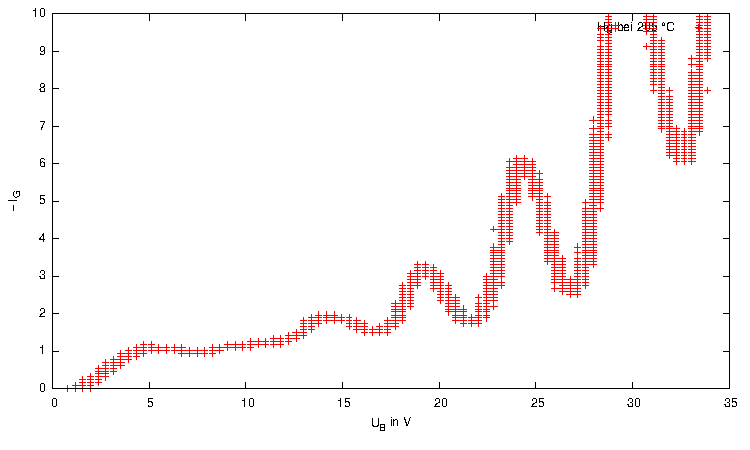
\includegraphics[width=\textwidth]{graphen/a2/a2c}}
\captionof{figure}{Erste für A3 aufgenommene Franck-Hertz-Kurve (\(T=185\,^\circ C\))}
\label{a2b}
\end{minipage}
\begin{minipage}{\linewidth}
\centering
\makebox[0cm]{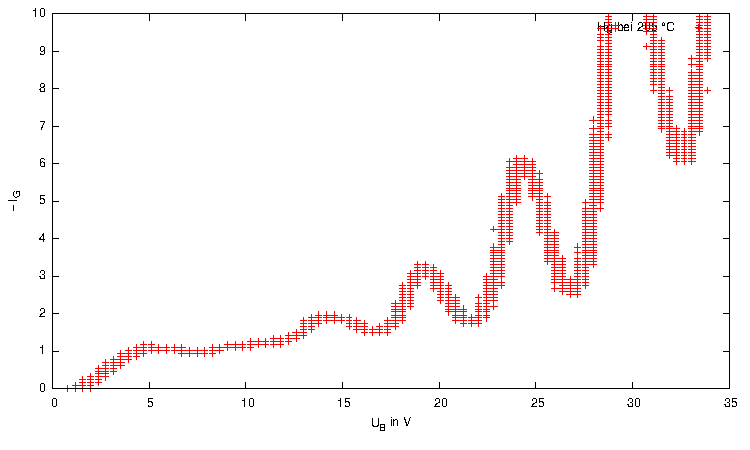
\includegraphics[width=\textwidth]{graphen/a2/a2c}}
\captionof{figure}{Erste für A3 aufgenommene Franck-Hertz-Kurve (\(T=205\,^\circ C\))}
\label{a2c}
\end{minipage}
\end{center}
Die so gefunden Spannungen \(U_B\) der Minima werden nun tabellarisch und anschließend mit einer linearen Regression dargestellt um die Steigung \(b\) des als linear angenommen Verlaufs zu erhalten.
\begin{center}
\begin{tabular}{c|c|c|c|c}
Minimum & \(T=190\,^\circ C\) & \(T=155\,^\circ C\) & \( T=185\,^\circ C\) & \(T=205\,^\circ C\)\\\hline
\(0\) & \(16,85\, V\) & \(11,85\, V\) & \(11,75\, V\) & \(16,50\, V\)\\
\(1\) & \(21,90\, V\) & \(16,85\, V\) & \(16,75\, V\) & \(21,50\, V\)\\
\(2\) & \(26,65\, V\) & \(21,80\, V\) & \(21,85\, V\) & \(26,80\, V\)\\
\(3\) & \(31,50\, V\) & \(27,00\, V\) & \(27,00\, V\) & \(32,35\, V\)\\
\(4\) & \(36,85\, V\) & \(-\) & \(-\) & \(-\)\\
\end{tabular}
\captionof{table}{Minima von \(U_B\) der aufgenommenen Franck-Hertz-Kurven}
\begin{minipage}{\linewidth}
\centering
\makebox[0cm]{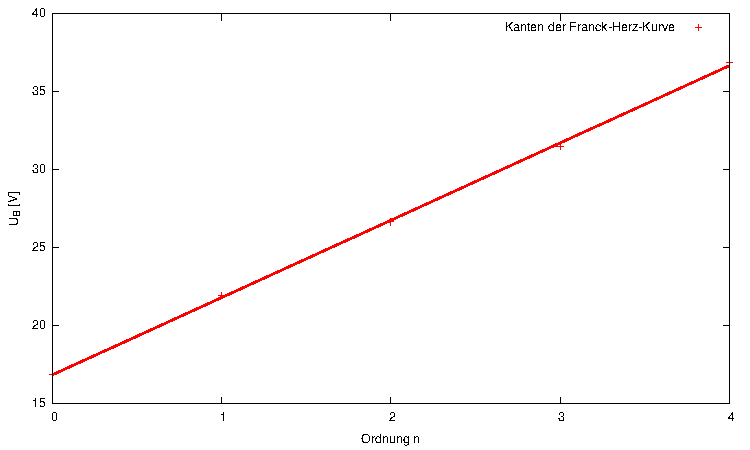
\includegraphics[width=\textwidth]{graphen/a1/graph}}
\captionof{figure}{Minima der Franck-Hertz-Kurve bei (\(T=190\,^\circ C\))}
\label{graph_a1}
\end{minipage}
\begin{minipage}{\linewidth}
\centering
\makebox[0cm]{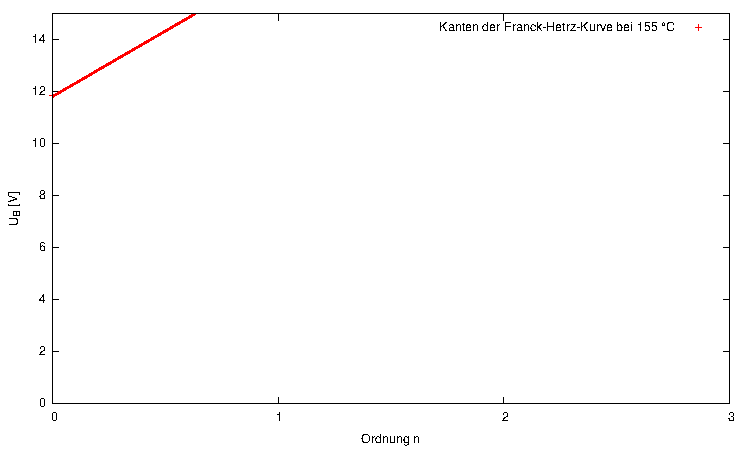
\includegraphics[width=\textwidth]{graphen/a2/graph_a}}
\captionof{figure}{Minima der Franck-Hertz-Kurve bei (\(T=155\,^\circ C\))}
\label{graph_a2a}
\end{minipage}
\begin{minipage}{\linewidth}
\centering
\makebox[0cm]{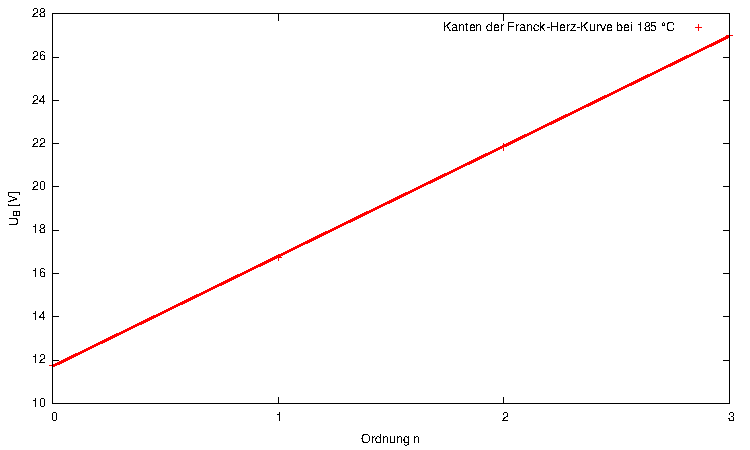
\includegraphics[width=\textwidth]{graphen/a2/graph_b}}
\captionof{figure}{Minima der Franck-Hertz-Kurve bei (\(T=185\,^\circ C\))}
\label{graph_a2b}
\end{minipage}
\begin{minipage}{\linewidth}
\centering
\makebox[0cm]{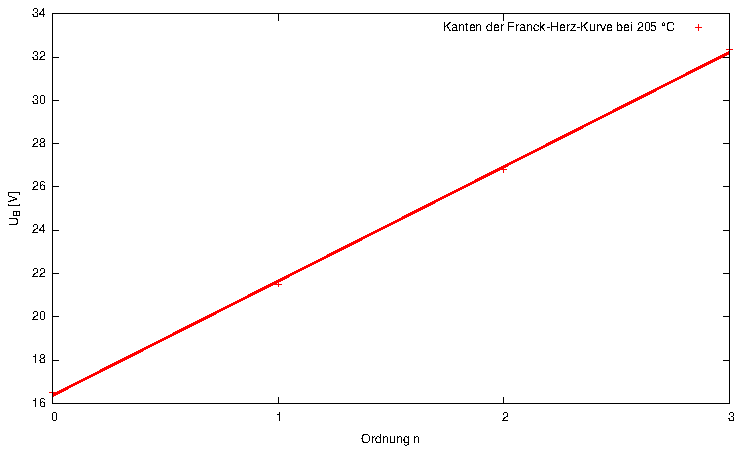
\includegraphics[width=\textwidth]{graphen/a2/graph_c}}
\captionof{figure}{Minima der Franck-Hertz-Kurve bei (\(T=205\,^\circ C\))}
\label{graph_a2c}
\end{minipage}
\end{center}
\newpage
Ermittelt wurden so folgende Steigungen:
\begin{center}
\begin{tabular}{c|c}
Temperatur \(T\) & Steigung \(b\)\\\hline
\(190\, ^\circ C\) & \(\left( 4,960 \pm 0,057 \right) \, V\) \\
\(155\, ^\circ C\) & \(\left( 5,040 \pm 0,038 \right) \, V\) \\
\(185\, ^\circ C\) & \(\left( 5,085 \pm 0,024 \right) \, V\) \\
\(205\, ^\circ C\) & \(\left( 5,285 \pm 0,087 \right) \, V\) \\
\end{tabular}
\captionof{table}{Die Steigungen der aufgetragen Minima}
\end{center}
\subsection{Auswertung}
Wie in den theoretischen Grundlagen erklärt, wechselwirken die Elektronen ab einer Bestimmten Energie mit den Quecksilberatomen und geben dabei ihre kinetische Energie ab. Durch Variation der Beschleunigungsspannung \(U_B\) konnte festgestellt werden, dass dies dazu führt, dass in bestimmten Intervallen der Gegenstrom \(I\) abbricht. Das ist erklärbar, denn verlieren die Elektronen ihre kinetische Energie kurz vor dem Gitter \(G\), so haben sie nicht mehr genügend Energie um das Gegenfeld zu passieren. Die Spannungsintervalle in denen das geschieht sind in unserem Fall genau die Steigungen \(b\) der gegen die Ordnung \(n\) aufgetragenen Minima. Die Energie der Elektronen, die mit einem Quecksilberatom wechselwirken entspricht genau der Energie, die sie durch das Elektrische Potential dieser Intervalle aufgenommen haben. daher gilt:
\begin{align}
E_{kin} &= \Delta U \cdot q \\
&= b \cdot e^-  \label{E_kin}
\end{align}
Die Spannungen lassen sich daher sehr einfach in Energien in \(eV\) umrechnen:
\begin{center}
\begin{tabular}{c|c}
Temperatur \(T\) & Anregungsenergie\(E_{Hg}\)\\\hline
\(190\, ^\circ C\) & \(\left( 4,960 \pm 0,057 \right) \, eV\) \\
\(155\, ^\circ C\) & \(\left( 5,040 \pm 0,038 \right) \, eV\) \\
\(185\, ^\circ C\) & \(\left( 5,085 \pm 0,024 \right) \, eV\) \\
\(205\, ^\circ C\) & \(\left( 5,285 \pm 0,087 \right) \, eV\) \\
\end{tabular}
\captionof{table}{Die Aufnahmeenergien von Quecksilber}
\end{center}
\subsection{Zwischenfazit}
Der Franck-Hertz-Versuch konnte mit der Quecksilberröhre  sehr gut durchgeführt werden, es ist zu sehen, dass sich bei verschiedenen Temperaturen die Anregungsenergie zu ändern scheint. Physikalisch erklärbar ist das von diesem Standpunkt aus aber nicht und es ist davon auszugehen, dass es sich wohl eher um Messfehler als um tatsächliche Effekte handelt. Außerdem ist der Fehler nur aus der Streuung der Messwerte errechnet worden, und da teilweise nur 4 Messwerte vorhanden waren ist dieser natürlicher klein, daher ist es auch möglich, dass der angegebene Fehler zu klein gewählt ist. Im Endergebnis steht:
\begin{center}
\begin{tabular}{c|c}
Temperatur \(T\) & Anregungsenergie\(E_{Hg}\)\\\hline
\(190\, ^\circ C\) & \(\left( 4,96 \pm 0,06 \right) \, eV\) \\
\(155\, ^\circ C\) & \(\left( 5,04 \pm 0,04 \right) \, eV\) \\
\(185\, ^\circ C\) & \(\left( 5,09 \pm 0,03 \right) \, eV\) \\
\(205\, ^\circ C\) & \(\left( 5,29 \pm 0,09 \right) \, eV\) \\
\end{tabular}
\captionof{table}{Die Aufnahmeenergien von Quecksilber}
\end{center}
Der Literaturwert liegt in etwa bei \(4,9\, eV\) und entspricht der  \(253\, nm\) Absorptionslinie des Quecksilbers, die im UV-Bereich liegt und damit nicht sichtbar ist. Es ist außerdem auch davon auszugehen, dass die Temperaturänderung nicht wie gewünscht verlaufen ist, da die Apparatur sehr träge auf Änderungen der Heizung reagiert, und nicht ausreichend Zeit war um hinreichend lange zu warten. Bei der Temperatur, die am längsten eingestellt war \(T=190^\circ C\), lieferte der Versuchsaufbau einen zum Literaturwert identischen Messewert.